\documentclass[aps, prb, twocolumn, a4paper, floatfix, reprint]{revtex4-2}
\usepackage[%
    margin=10mm,% ако не си принтира 10мм не изглежда грозно, а може да събереш повече текст
    % showframe=true,%
    ]{geometry}
\usepackage[T1,T2A]{fontenc}
\usepackage[utf8]{inputenc}
\usepackage[main=bulgarian, english]{babel}
\usepackage{float}
\AtBeginDocument{\selectlanguage{bulgarian}}
\newcommand{\degree}{^{\circ}}
\usepackage{amsmath}
\usepackage{graphics}
\usepackage{graphicx}
\graphicspath{{.}}
\newcommand{\abs}[1]{\lvert#1\rvert}
\let\phi\varphi
\usepackage{booktabs} % от тук се използва само \midrule може и без него 
%\usepackage{adjustbox} % това може да се използва, за да „смаляваш“ широки таблици
%\usepackage{tabularx} % дефинира колона X в среда tabularx която добавя празно място така че цялата таблица да запълни определена ширина
\usepackage{dcolumn}
\newcolumntype{d}[1]{D{.}{.}{#1}}
\usepackage[unicode=true,pdfusetitle]{hyperref}


\makeatletter
\renewcommand{\Dated@name}{}%
\makeatother



\begin{document}
\title{Термодвойка}
\author{Васил Николов}
\noaffiliation
\date{08.03.2022}
\maketitle

\section{Цел на упражнението}
Да се наблюдава втвърдяването на смес на Вуд, и да се изследва и калибрира термодвойка, потопена в сместа. 

\section{Експериментална установка}
Едната част на диференциална термодвойка е потопена в термос с вода и лед, а другата - в колба съдържаща сплав на Вуд. Върху сплавта е изсипан глицерин, за да се избегне окисляване, и цялата колба е потопена във вода, която може да се нагрява от котлон. Термодвойката е свързана към усилвател на напрежението, който го превръща в сигнал от порядъка на десетки миливолти, който може да се измери с мултицет с точност $\delta U_0 = 0.1 \ mV$. Тъй като единият край на термодвойката е потопен в среда с температура $T_0 = 0^{\circ}C$, то напрежението от усилвателя отговаря на температурата на сместа в целзиеви градуси. След като колбата със сместа се нагрее до $T_{max} = 92^{\circ} C$ котлонът се премахва и сместа се охлажда. Правят се измервания докато се стигне до $T_{min} = 52^{\circ} C$, като в този температурен интервал е и температурата на фазофия преход на сместа на Вуд, около $T_{ph} = 69^{\circ} C$. За калибрация на термодвойката се използва живачен термометър, който също е потопен в сплавта. 

\section{Теоретична обосновка}
\subsection{Градуиране на термодвойката}
Заради неидеалност на усилвателя и ефекта на Зийбек не може да очакваме идеална зависимост на термоелектродвижещото напрежение от разликата в температурите. 
\begin{gather*}
    U_{ideal} = K\Delta T \\
    U_{real} = a\Delta T^2 + b\Delta T + c
\end{gather*}
Измереното термоелектродвижещото напрежение се приближава с полином от втора степен защото по-високи степени не добавят точност в модела. 

\subsection{Фазов преход на сплав на Вуд}
При охлаждането на сместа очакваме експоненциално намаляване на температурата до достигането на фазовия преход, плато на температурата при температурата на фазовия преход и отново експоненциално намаляване след него. Следователно очакваме функцията на температурата от времето да е следната
\begin{equation*}
    T(t) = \begin{cases}
        T_r + (T_0 - T_r) e^{-\lambda t} \quad \text{for } t < t_1 \\
        T_{ph} \quad \text{for } t_1 < t < t_2 \\
        T_r + (T_{ph} - T_r) e^{-\lambda (t - t_2)} \quad \text{for } t > t_2
    \end{cases} 
\end{equation*}
Тук $T_r$ е стайната температура. 

\section{Експериментални данни и резултати}
\subsection{Градуиране на термодвойката}
На графиката са представени измерените стойности за термоелектродвижещото напрежение като функция на температурата, както и най-добре описващата ги парабола. 

\begin{figure}[H]
    \centering
    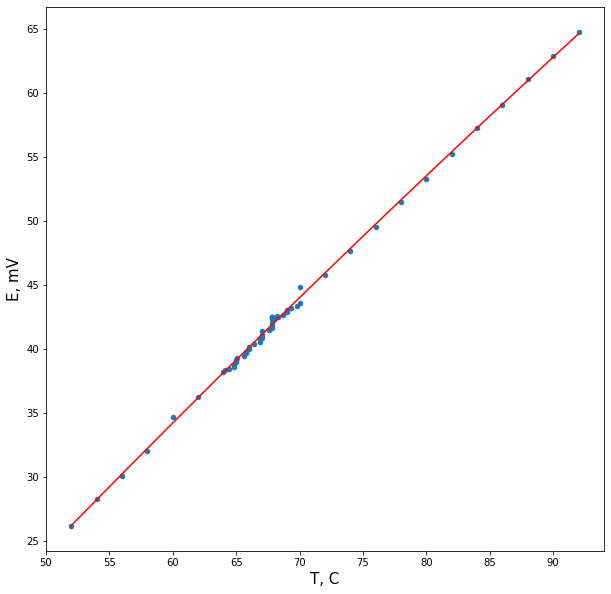
\includegraphics[width=0.9\columnwidth, keepaspectratio=true]{graduirane.png}
\end{figure}

Параметрите на калибровъчната крива са 
\begin{equation*}
    a = -1.296.10^{-3} \frac{mV}{K^2}, \ b = 1.147 \frac{mV}{K}, \ c = -29.89 mV
\end{equation*}
Съобразявайки в коя част на парабобата е интервалът на измервания можем да пресметнем офратната функция 
\begin{equation*}
    T = T(E) = \frac{-b+\sqrt{b^2 - 4a(c-E)}}{2a}
\end{equation*}

Грешката при определяне на температурата по този начин е 
\begin{equation*}
    \delta T = \sqrt{T_{rmse}^2 + (\frac{\delta U_0}{b})^2} = 0.3K
\end{equation*}
Тук $T_{rmse}$ е средната квадратична грешка на пресметнатата температура. 

\end{document}